\section{Sensoren}\label{sec:Sensoren}

% Hinweis auf C-Code, Verweise auf Kapitel von olliver, nur Besonderheiten hier erwähnt

% Überall noch Daten aus Präsentation einbringen, eventuell kleine Tabellen, nicht zwingend

% Verweis auf Strom und Spannungsmessung (das haben wir schon, Rest kommmt JETZT)

\subsection{Kompassmodul QMC5883L}

Als Kompass dient uns der \textbf{QMC5883L}. Verwendet wird er, um die Ausrichtung der Wetterstation gen Norden zu messen. Diese Information wird benötigt, um das Solarpanel korrekt zur Sonne auszurichten zu können. 

% Mehr blabla aus Datenblatt, 3 Achsen etc pp. Ding soll ja verkauft werden

Mit einer Genauigkeit von \ang{1} bis \ang{2} ist er für unsere Zwecke ausreichend genau. Ebenfalls für den Sensor sprechen seine geringe Stromaufnahme von 75\,$\mu$A und die Möglichkeit ihn mittels I\textsuperscript{2}C anzusprechen. 

\subsubsection{Montage}

Das Kompassmodul hat 5 Anschlüsse, von denen wir vier verwenden: V\textsubscript{CC}, GND, SDA und SCL. Der fünfte Anschluss wird nur bei einer häufigen Datenübertragung benötigt, er sendet die Information, dass Daten zum Abruf bereit stehen. Dargestellt ist die Verschaltung in Abbildung~\ref{fig:QMC5883L_Plan}.

\begin{figure}[H]
  \centering
  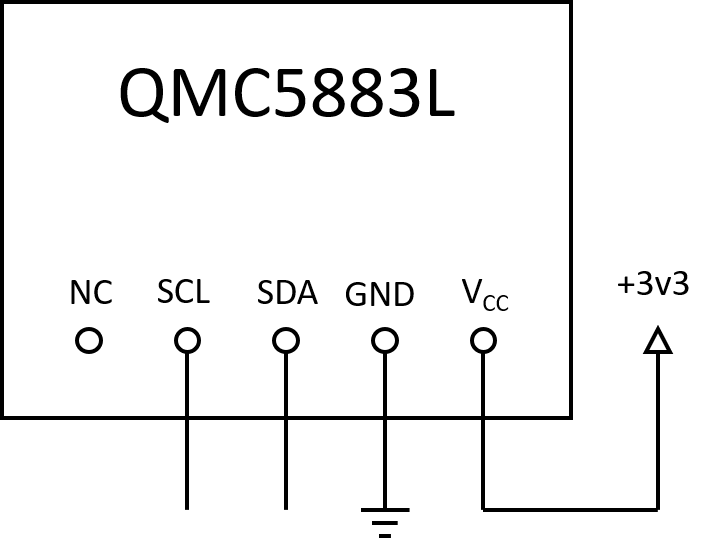
\includegraphics[width=0.4\textwidth]{./img/QMC5883L_Plan.png}
  \caption{Verschaltung des QMC5883L}\label{fig:QMC5883L_Plan}
\end{figure}

Da der Sensor das Magnetfeld misst, muss dieser entfernt von der Windfahne und dem Anemometer platziert werden, da beide mit magnetischen Bauteilen arbeiten. Andernfalls könnte es zu Fehlmessungen kommen. Umgesetzt wurde dies so, dass an der einen Stütze des Solarpanels das Kompassmodul und an der anderen die Windfahne, das Anemometer und das gegenüber magnetischen Beeinflussungen relativ unempfindliche GPS-Modul angebracht wurden.

% Verweis auf noch einzufügendes Bild der Montage

%\begin{figure}[H]
% \centering
%  \includegraphics[width=\textwidth]{./img/Montage.png}
%  \caption{Verschaltung des QMC5883L}\label{fig:Montage}
%\end{figure}

\subsection{GPS} % richtiges Datenblatt finden und Werte einsetzen56tr

Um den Standort des Geräts zu bestimmen und auch um die Berechnung der korrekten Auslenkung des Solarpanels auf Grund des Standorts zu ermöglichen, musste ein GPS-Modul genutzt werden. Wir haben uns für den % Gerätetyp entschieden. Er ermöglicht eine Bestimmung der aktuellen Position um XX m in der Horizontalen und um XX in der Höhe.

\subsubsection{Montage}

Da das GPS-Modul in Einheit mit einer Antenne funktioniert, musste das Modul entfernt von der Elektronik und damit außerhalb des Gehäuses platziert werden. Dazu bot sich an, das GPS-Modul an der zweiten Stütze des Solarpanels zu platzieren. Das Modul wurde dafür ebenso in einem Nebengehäuse untergebracht (s. Kap.~\ref{sec:ge_neben}). Die Antenne des Moduls wurde dabei mittels Kabelbinder an der Stütze angebracht. Dieses Vorgehen war einer dauerhaften Anbringung, etwa durch Kleber, vorzuziehen, da die Bauteile so leichter ausgetauscht werden können.

% Bild Anschlüsse

\subsection{Anemometer und Windfahne}

% Vorgänger wegen seriell und so doof
% neues Modell mit Doku, andernfalls reverse Ingeneering
% Funktion


\subsubsection{Montage}

% Position

% Bild Anschlüsse

% Bild Montage

\subsection{Neigungssensor MPU6050}

% Zweck, Bestimmung Neigung des Panels, Feedback für Motor

\subsubsection{Montage}

\begin{figure}[H]
  \centering
  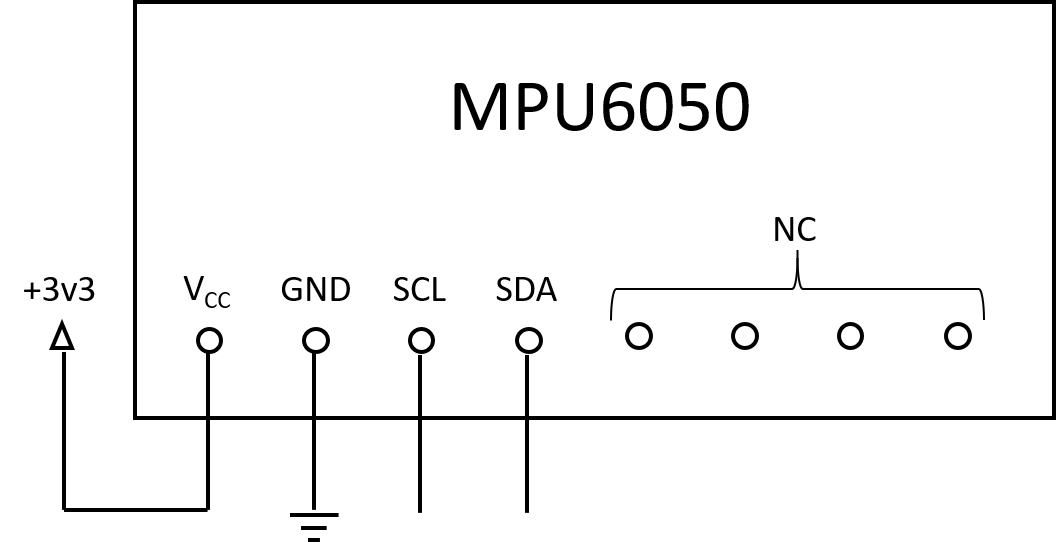
\includegraphics[width=0.6\textwidth]{./img/MPU6050_Plan.png}
  \caption{Verschaltung des MPU6050}\label{fig:MPU6050_Plan}
\end{figure}

\subsection{BME280}

% Zweck, Genauigkeit, Arbeitsbereich

\subsubsection{Montage}

% Wo ist der? Im Gehäuse? Bild!

\begin{figure}[H]
  \centering
  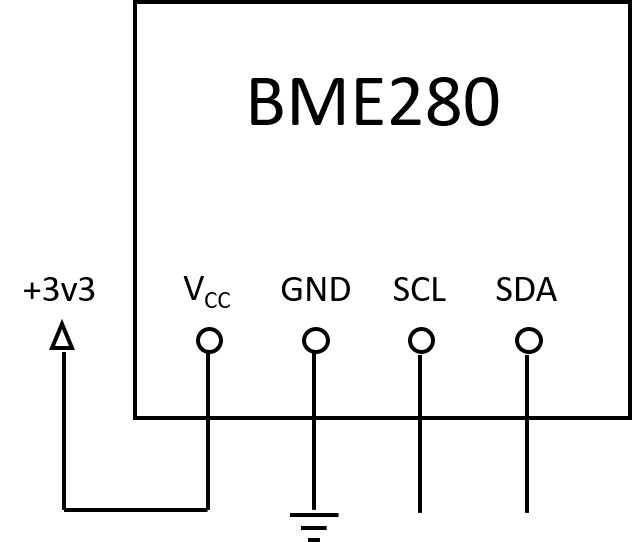
\includegraphics[width=0.4\textwidth]{./img/BME280_Plan.png}
  \caption{Verschaltung des BME280}\label{fig:BME280_Plan}
\end{figure}

\subsection{Anschlagssensor}

% Zweck, Positionierung Panel, noch von Vorgängern, Schutz Motor und Teile. Funktion

\subsubsection{Montage}

% an Achse des Panels

% Verkabelung erklären

